% This is LLNCS.DOC the documentation file of
% the LaTeX2e class from Springer-Verlag
% for Lecture Notes in Computer Science, version 2.4
\documentclass{llncs}
%\usepackage{llncsdoc}
%
\usepackage[T1]{fontenc}
\usepackage[utf8]{inputenc}

\usepackage{cite}
%\usepackage {natbib}
\usepackage{graphicx}
\usepackage{multirow}

\begin{document}

\title{Fuzzy Simulation of Human Behaviour in the Health-e-Living System}

\author{Remberto Martinez\inst{1} \and Marcos Tong\inst{1} \and Luis Diago\inst{2,3} \and Timo Nummenmaa\inst{4} \and Jyrki Nummenmaa \inst{4}}

\institute{
ExtensiveLife Oy, Lohkaretie 2 B 9, 33470 Tampere, Finland
\and
Interlocus Inc, Yokohama City 226-8510, Japan
\and 
Meiji Institute for Advanced Study of Mathematical Sciences\\ Meiji University, 4-21-1 Nakano, Tokyo 164-8525, Japan
\and 
University of Tampere, Finland}

\maketitle
%
\begin{abstract}

This chapter shows an application of fuzzy set theory to preventive health support systems where adherence to medical treatment is an important measure to improve health, and reduce health care costs. Current health care information technology (health-IT) systems focus on ensuring adherence to medication through Just- In-Time Adaptive Interventions (JITAI). Determining the timing of the intervention and the appropriate intervention strategy are two of the main difficulties facing current systems. In this work, a JITAI system called Health-e-living (Heli) was developed for a group of patients with type-2 diabetes. During the development stages of Heli it was verified that the state of the action of each user is fuzzy and it is difficult to get the right moment to send motivational message without being annoying. A fuzzy formula is proposed to measure the adherence of patients to their goals. The effectiveness of interventions is essential in any JITAI system and the proposed formula allows Heli to send motivational messages in correspondence with the status of each user as to evaluate the efficiency of any intervention strategy.. 

\end{abstract}

\keywords{JITAI, Behaviour analysis, Fuzzy measures}
%

\section{Introduction}
%

Preventive health support systems...

Fuzzy set theory...
 
In the work presented at ISFUROS 2017 we have a fuzzy modeling to calculate progress and to send motivation emails to users depending on the type of adherence to the system (high, medium or low). The types of data that are acquired are related to nutrition, physical activity mainly. However, the results ware only preliminary because the sample size is not large and there were a lot of missing data. In this chapter we add the Fuzzy Simulation of User's Behavior with missing data in order to validate our previous modeling by Fuzzy Rules extraction from Time Series and using rules to reproduce real models and extract new knowledge from the simulations. We will include mainly three points:
\begin{itemize}
\item a) As the data we have in the Heli are very few, we use the Disco simulator~\cite{Disco} to reproduce our previous results through simulation.
\item b) We add the HAPA model~\cite{MacPhail} to the simulator and included fuzzy rules extracted from the adherence formula developed in our previous work.
\item c) We compare the results with those reported in~\cite{Brailsford2016} to demonstrate the advantages of modeling human behavior using fuzzy rules extracted from adherence data and to see if the simulation discovers a new user behavior or a new user type that is not registered in the system or in the literature.
\end{itemize}

The rest of the chapter is organized as follows. First, section \ref{sec.heli} introduces the Heli system, our previous fuzzy formula for measuring user's adherance to de system and the modeling of Human Behavior with a simplified HAPA model. Section \ref{sec.helimodel} briefly describes the Disco simulator and introduces the developed simulation of Human behaviour in Heli. Section \ref{sec.rules} presents the proposed method to extract rules from the simulations and section \ref{sec.results} compare the results with those reported in~\cite{Brailsford2016} to demonstrate the advantages of modeling human behavior using fuzzy rules extracted from adherence data. Finaly, conclusions and future works are presented in section~\ref{sec.conclusions}

\section{Health-e-living (Heli) System}
%
\label{sec.heli}

 Health-e-living (Heli)\cite{rem2012} is a mobile solution to deliver preventive, educational and promotional health to all citizens comfortable with IT technologies independently of their age or geographical location. Heli uses the metaphor of social networks to improve health habits of persons connected to their support network in real life (family, friends, and colleagues). Figure~\ref{Fig.heli} shows the logical solution provided by the Heli system.
\begin{figure}
  \begin{center}
  \begin{tabular}{c}
    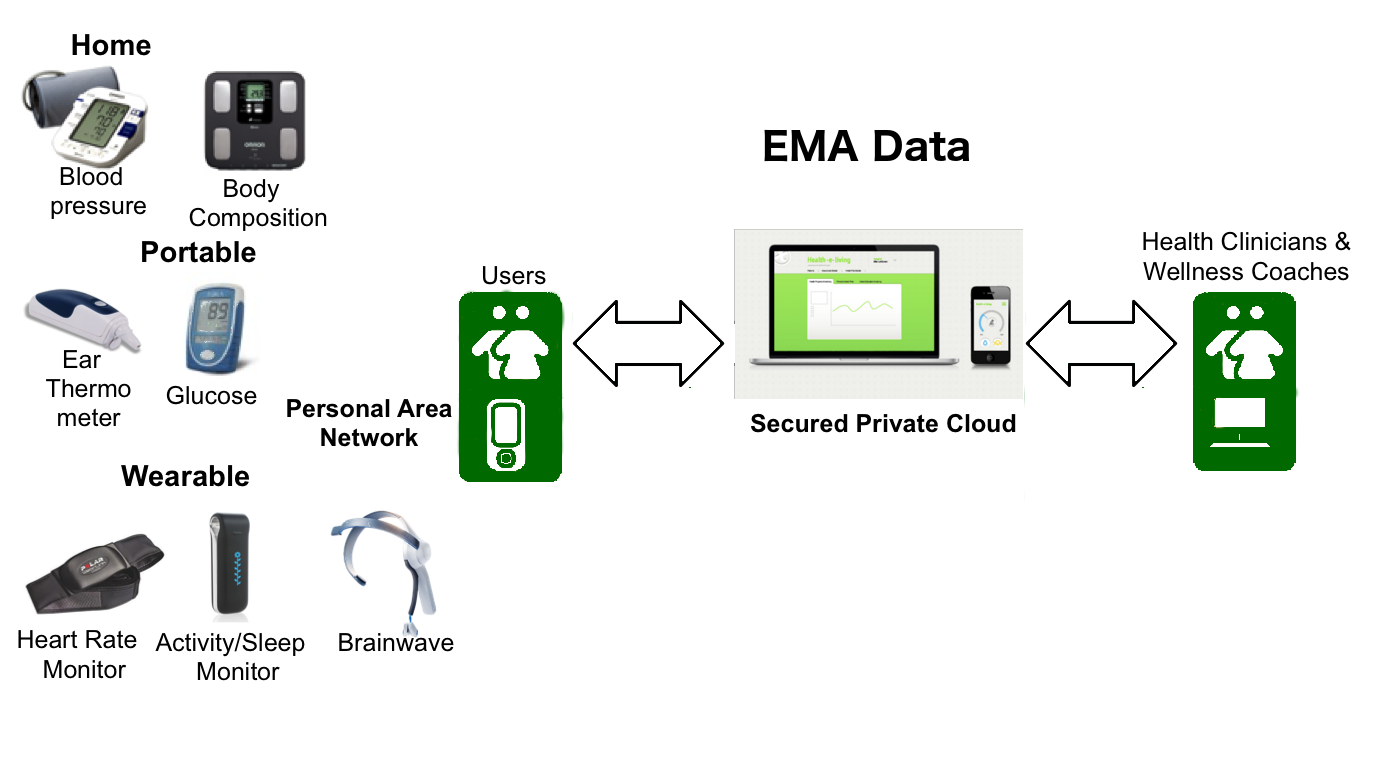
\includegraphics[scale=0.5]{LogicalSolutionNow.png}\\
    \end{tabular}
    \caption{Logical Solution provided by the Heli system\cite{rem2012}}
     \label{Fig.heli}
\end{center}
\end{figure} 

\subsection{Fuzzy  Adherance Measurement}

People's health determinants are difficult to model because of their inherent uncertainty, the complex interactions among them, as well as the considerable number of variables and lack of precise mathematical models. This was the main motivation to use a fuzzy approach as a  practical option to model the adherence to a treatment and healthy lifestayle of a patient in the Heli system. In Heli, two variables are combined for the evaluation of patients' status: the progress of the proximal outcomes $\Delta x = \|x - g_i\|$  and the patient adherence to the system $y = F(x,z)$. Note that the value of $y$ depends on the inputs $x$ (i.e. proximal outcomes) which are controlled by the patients and the contextual inputs $z$ (e.g. environment) which are not controlled by the patients. Progress indicates how close a patient is to completing the outcomes $g_{i(1\leq i \leq n)}$ and the adherence measures how effective the system is in its intervention. The adherence is modeled as a fuzzy weighted average involving type-1 (T1) fuzzy sets as follows~\cite{Liu2008}:
\begin{equation}
y = \frac{\sum_{i=1}^n w_i x_i}{\sum_{i=i}^n w_i}
\label{Eq.AdheranceFWA}
\end{equation}
In (\ref{Eq.AdheranceFWA}), $w_i$ are weights that act upon proximal outcomes $x_i$. While it is always true that the sum of the normalized weights that act upon each $x_i$ add to one, it is not a requirement that the sum of the unnormalized weights must add to one. The adherence is calculated as an average of several goals, and gives an idea of how well the system goes with the goals of the patients. Every goal $g_i$ is defined on an interval $g_i \in [g_{-}, g^{+}]$ and the values of $y_{-}$ and $y^{+}$ are computed accordingly as follows:
\begin{equation}
 	y_{-}(x)= \left\{ 
	\begin{array}{lcr}
        1,	         & if &(x \geq g_{-})\\
        x/g_{-} 	 & if &(0<x<g_{-})\\
        1                & &otherwise
	\end{array}
	\right \},
 	y^{+}(x)= \left\{ 
	\begin{array}{lcr}
        1,	         & if &(x \leq g^{+}),\\
        \frac{2g^{+}- x}{g^{+} }	 & if &(g^{+}<x<2g^{+} )\\
        0                & if & x \geq 2g^{+}\\
        1                & & otherwise
	\end{array}
	\right \}.
\label{Eq.Adherance}
\end{equation}
As it was mentioned before, the choice of the time interval between decision points can have a dramatic impact on the ability of the adaptation to achieve its goals. Patient progress is calculated daily and adherence is added to the system weekly but it is calculated every two weeks because we can not calculate without data. The time interval between decision points is set to two-weeks to see how many entries there are in that period. As long as adhesion is closer to 1 the system is more effective.

\subsection{Modeling Human Behavior with a simplified HAPA model}

HAPA is designed as a sequence of two continuous self-regulatory processes, a goal-setting phase (motivation) and a goal-pursuit phase (volition). The second phase is subdivided into a pre-action phase(volition) and an action phase(maintenance) (see~Fig.\ref{fig.hapa}

\begin{figure}
  \begin{center}
  \begin{tabular}{c}
    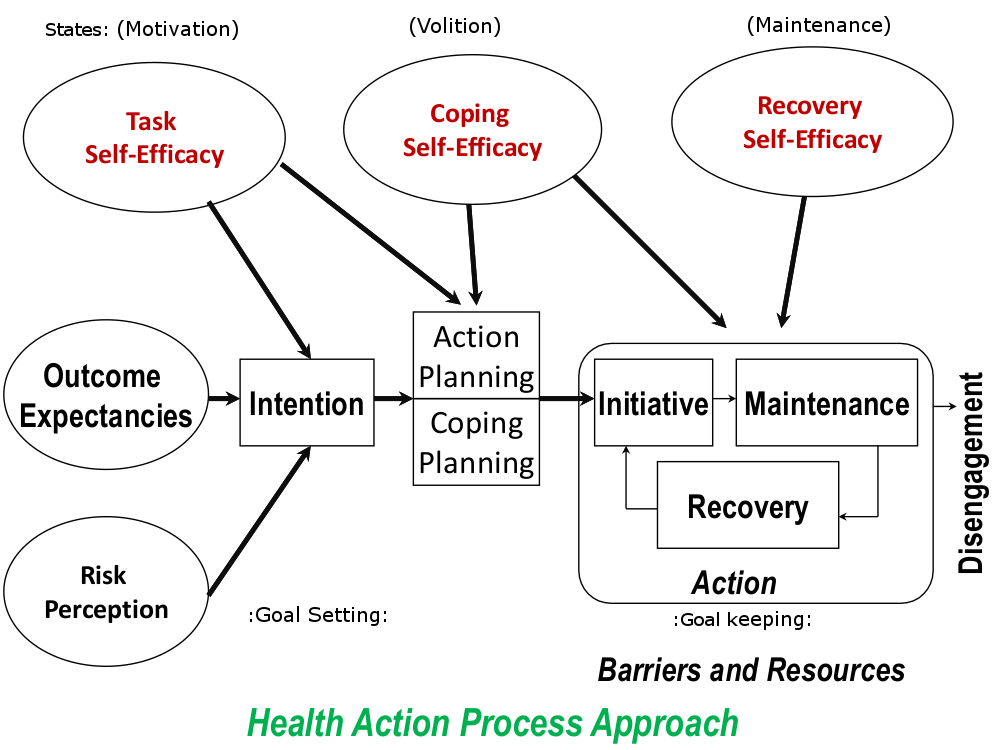
\includegraphics[scale=0.5]{hapa_firem.png}\\
    \end{tabular}
    \caption{Hapa \cite{rem2012}}
     \label{Fig.hapa}
\end{center}
\end{figure} 

In this work we use the stage model; the stage approach assumes that change is non-linear and consists of several qualitative steps that reflect different mindsets of people.
We could model the efficacy of HeLi as the probability of compliance with Health Goal set at the evaluation time ( 2 weeks ) or just simply the probability of compliance with an intended Health Behavior Change.

\begin{equation}
 	HBC(t) =  AH(t) * MA(t) * P(t)
\label{Eq.HBChange}
\end{equation}


Where AH is adherence history over the time the system is used = ( A - 0.1x \# of inputs ) MA is Motivation to comply with Health Goal selected =  Mi x Bi, (motivation + beliefs ) P is the Perceived Self-Efficacy =  Ok x Rk ( outcomes expectations + risk perception)
Brailsford used a probability to participate in treatment of 0.85 [2], which is equivalent in this work to the probability of any user to input data after selecting a personal goal. Assuming that motivation to provide personal data is constant for all users, it is possible to model three main users types influenced by the normative believe that entering data in the system will contribute to achieving their goal as low ( 0.5), medium (0.8) and high (1.0) and that will lead to provide more entries during the time span of two weeks. It is possible to assume in a first phase that P is always 1.
With this simplistic model can have simulated data to represent equivalent results to those obtained in real data. In this model the simulator should be configured to generate an input event based on certain probability. In this first iteration the user behavior is able to form an intention, plan and take basic actions. The next step would be to model a user behavior that is influenced by the environment and will change the perceived self-efficacy in time.
The main contribution HAPA model is allowing perceived self-efficacy to change over time in situations where user needs to cope with setbacks or recover from life challenges. In this iteration is possible to add two more properties to the user model:emotional commitment ( 1, can cope or 0.1, not ) and failure learning ( 1, can recover or 0.2, not ). Now the simulated data allows a user to react on the event of receiving a motivational message or not. In this phase the value of P will be calculated over time.

As the data we have in the Heli are very few and there is a lot of missing data, in this chapter we add the Fuzzy Simulation of User's Behavior in order to validate our previous modelling.

\section {Simulation of Human Behaviour in Heli System}
\label{sec.helimodel}
The main purpose of simulating Human Behaviour was to validate the adherence formula used in Heli system by generating equivalent data to the one observed for a period of time in real runtime of Heli system presented in paper [ISFUROS2017].
Adherence to the system is observed as the number of data inputs during a week period of time. Assuming all users has already registered to the system and defined a goal ( on targets related to weight management, better nutrition and increase physical activity level), when no entries available about user’s activity EMA ( Ecological Momentary Assessment on the topics weight, nutrition or physical activity ) we can consider the user is in HAPA\_Motivational state. At the same time if EMA entries are available the user is considered in HAPA\_Volitional or HAPA\_Maintenance state and the contents of each entries can be used to calculate the progress over time towards the selected goal (see Fig.\ref{Fig.hapa}).
Over the elapsed time in the simulated world environment, every two weeks is possible to assess the value of adherence and based on that the system sends personalized messages according to user attribute compliance: not\_very\_active, active and very\_active. For simulation purposes it is possible to define an additional user attribute representing resilience. Resilience can be simplified to include user’s emotional commitment and the ability to learn from failure as a user being of two types: responsive and not\_responsive. A user being responsive will have a high correlation with user in HAPA\_Volitional or HAPA\_Maintenance states, being active or very\_active. The user model does not include the persuasive element as this is an attribute of the system and not of the user behavior.
Figure~\ref{Fig.hapa} shows ...
\begin{figure}
  \begin{center}
  \begin{tabular}{c}
    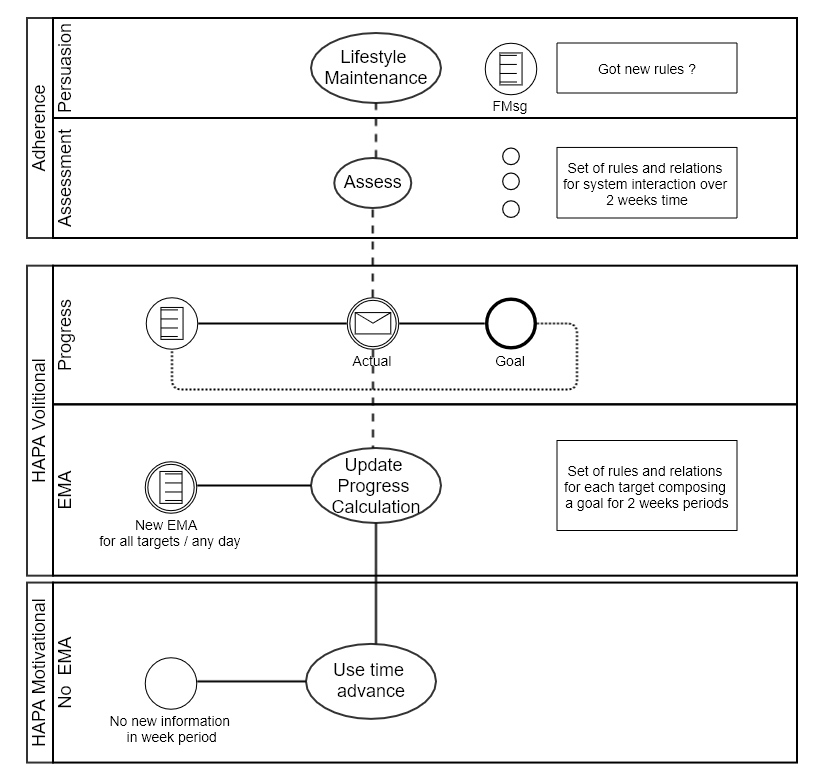
\includegraphics[scale=0.5]{Hapa.png}\\
    \end{tabular}
    \caption{...}
     \label{Fig.hapa}
\end{center}
\end{figure} 

\section {Fuzzy Rules extraction from Time Series}
\label{sec.rules}
by Fuzzy Rules extraction from Time Series and using rules to reproduce real models and extract new knowledge from the simulations

\section {Preliminary Results}
\label{sec.results}

\vspace*{-\baselineskip}\vspace*{-\baselineskip}\vspace*{-\baselineskip}\section {Conclusions and Future Works}
\label{sec.conclusions}

%JITAI systems like Heli appear to be a promising framework for developing mHealth interventions; however, this research is still in its infancy. Fuzzy measures like the proposed adherence formula constitute a practical option to model phenomena with the inherent uncertainty. Machine learning can be also a potent tool to enhance the effectiveness of a JITAI based computational models of human behavior like the health action process approach (HAPA)\cite{MacPhail}.
%JITAI systems like Heli appear to be a promising framework for developing mHealth interventions. In Heli, the number of users with fuzzy adherence was very small (25/98 $\approx$ 25.5\%) because most users (73/98 $\approx$ 74.5\%) prefer to use the system to store daily data without a specific goal. However, the  proposed interventions showed that even after several stress inputs patients do not leave the system. Although this research is still in its infancy, fuzzy measures like the proposed adherence formula constitute a practical option to model phenomena with the inherent uncertainty like the patient state measurement. As the emotional dimensions used in the research may not be the most adequate, we are currently pursuing researches to use machine learning tools to enhance the effectiveness of Heli based on computational models of human behavior like the health action process approach (HAPA)\cite{MacPhail}.

% --------------
% 101 - do not send more messages --- desinterest
% 102 - keep up the good work --- maintenance
% 103 - prime to change --- motivation
% 104 - physical activity increase ---maintenance
% 105 - moderate active everyday life --- maintenance
% 106 - reduce sedentary time --- maintenance
% 107 - vegetables and fruits --- maintenance
% 108 - better proteins --- maintenance
% 109 - good carbs --- maintenance
% 110 - regular meal pattern --- maintenance
% 111 - healthy fats --- maintenance
%
% En los estados nuevos estan relacionados los goals directamente.
% Rem : Me interesa sacar la probabilidad de que un usuario se mueva de un estado a otro.
% Por ejemplo: del 103 al 104...109 y entre 104...109 puede saltar librement
% el 101 es muy dificil moverlo porque esta desinteresado
% y el 102 porque esta muy bien y no necesita ningun cambio
% del 103 al 109 son los estados que demuestran apego al sistema
% El sistema viejo es mas rectivo/retrospectivo
% El sistema nuevo es mas predictivo
%

%After several stress inputs patients do not leave the system.

%Most users (73/98 = 74.5\%) prefer to use the system to store daily data without a specific goal.

%The emotional dimensions selected were not the most adequate

\begin{thebibliography}{99}
\bibliographystyle{splncs}

\bibitem{Disco} The DisCo project WWW page. At URL http://disco.cs.tut.fi on the World Wide Web.

\bibitem{Brailsford2016} Brailsford S.C. Healthcare: Human Behavior in Simulation Models. In: Kunc M., Malpass J., White L. (eds) Behavioral Operational Research. Palgrave Macmillan, London

\bibitem{Murray2016} Tylar Murray, Eric Hekler, Donna Spruijt-Metz, Daniel E. Rivera1, and Andrew Raij.: Formalization of Computational Human Behavior Models for Contextual Persuasive Technology, PERSUASIVE 2016, LNCS 9638, pp. 150?161, 2016. DOI: 10.1007/978-3-319-31510-2 13

\bibitem{Wan} Wai Yin Lam and Paula Fresco.: Medication Adherence Measures: An Overview. BioMed Research International Volume 2015, Article ID 217047, 12 pages doi: 10.1155/2015/217047

%\bibitem{Sidorkiewicz} Stephanie Sidorkiewicz, Viet-Thi Tran, Cecile Cousyn, Elodie Perrodeau, and Philippe Ravaud: Development and validation of an instrument to assess treatment adherence for each individual drug taken by a patient, 

\bibitem{Prado} Carlos A Prado-Aguilar, Yolanda V Martinez, Yolanda Segovia-Bernal, Rosendo Reyes-Martnez and Raul Arias-Ulloa Performance of two questionnaires to measure treatment adherence in patients with Type-2 Diabetes, BMC Public Health. 2009 Jan 26;9:38. doi: 10.1186/1471-2458-9-38.

%\bibitem{guidebook} Facilitating Treatment Adherence: A  Practitioner's Guidebook

\bibitem{Nahum-Shani} Inbal Nahum-Shani, \& Shawna N. Smith,  \& Bonnie J. Spring,  \&Linda M. Collins,  \& Katie Witkiewitz,  \& Ambuj Tewari, \& Susan A. Murphy, Just-in-Time Adaptive Interventions (JITAIs) in Mobile Health: Key Components and Design Principles for Ongoing Health Behavior Support, Annals of Behavioral Medicine 2016, doi: 10.1007/s12160-016-9830-8

\bibitem{rem2012} Remberto Martinez and Marcos Tong: Can Mobile Health Deliver Participatory Medicine to  All Citizens in Modern Society? 4th International Conference on Well-Being in the Information Society, WIS 2012, Turku, 22 August 2012 - 24 August 2012 Pages 83-90

\bibitem{Hafezi} Hooman Hafezi, Timothy L. Robertson, Greg D. Moon, Kit-Yee Au-Yeung, Mark J. Zdeblick, and George M. Savage, An Ingestible Sensor for Measuring Medication Adherence. IEEE Trans ON Biomedical Engineering, Vol. 62, No. 1, JANUARY 2015, pp 99-109

\bibitem{Nguyen} Thi-My-Uyen Nguyen, Adam La Caze \& Neil Cottrell, What are validated
self-report adherence scales really measuring?: a systematic review. British Journal of Clinical Pharmacology, 77:3 / 427?445

\bibitem{Hall2015} Amanda M. Hall, Steven J. Kamper, Marian Hernon, MPH,a Katie Hughes,  Chris Lonsdale, Deirdre A. Hurley and Raymond Ostelo, Measurement Tools for Adherence to Non-Pharmacologic Self-Management Treatment for Chronic Musculoskeletal Conditions: A Systematic Review, Arch Phys Med Rehabil. 2015 Mar;96(3):552-62. doi: 10.1016/j.apmr.2014.07.405.

\bibitem{MacPhail} Mariana MacPhail, Barbara Mullan, Louise Sharpe Carolyn MacCann and Jemma Todd Using the health action process approach to predict and improve health outcomes in individuals with type 2 diabetes mellitus. Diabetes, Metabolic Syndrome and Obesity: Targets and Therapy 2014:7 469?479

\bibitem{Liu2008} Feilong Liu,  and Jerry M. Mendel, Aggregation Using the Fuzzy Weighted Average as
Computed by the Karnik-Mendel Algorithms, IEEE Trans. on Fuzzy Systems, Vol. 16, No. 1, pp-1 - 12 

\bibitem{WEKA} M. Hall, E. Frank, G. Holmes, B. Pfahringer, P. Reutemann, I.H. Witten, The WEKA Data Mining Software:
An Update, SIGKDD Explor Newsl. 11 (2009) 10?18. doi:10.1145/1656274.1656278.

\end{thebibliography}


\end{document}